\documentclass[
10pt, % Set the default font size, options include: 8pt, 9pt, 10pt, 11pt, 12pt, 14pt, 17pt, 20pt
%t, % Uncomment to vertically align all slide content to the top of the slide, rather than the default centered
aspectratio=169, % Uncomment to set the aspect ratio to a 16:9 ratio which matches the aspect ratio of 1080p and 4K screens and projectors
]{beamer}

\usepackage[all]{xy}

\usepackage[spanish]{babel}
\usepackage[utf8]{inputenc}

\graphicspath{{Images/}{./}} % Specifies where to look for included images (trailing slash required)

\usepackage{booktabs} % Allows the use of \toprule, \midrule and \bottomrule for better rules in tables

%\usepackage{tikz}
%\usetikzlibrary{positioning}
%\usetikzlibrary{shapes,arrows,arrows,positioning,fit}

\usepackage{tikz}
\usetikzlibrary{mindmap}
\usetikzlibrary{arrows, positioning}
\usetikzlibrary{arrows, shapes, positioning, shadows, trees}

\usepackage{forest}

\usepackage{multirow}

\usepackage{graphicx}
\usepackage{hyperref}

\usepackage{xcolor,listings}
\usepackage{textcomp}
%\usepackage{color}

\usepackage{enumitem}

\usepackage{xcolor}

\usepackage{verbatim}
\usepackage{changepage}

\usepackage{algpseudocode}
\usepackage{gensymb}

\usepackage{venndiagram}

\usepackage{graphicx}


\providecommand{\abs}[1]{\lvert#1\rvert}

%----------------------------------------------------------------------------------------
%	SELECT LAYOUT THEME
%----------------------------------------------------------------------------------------
\usetheme{Madrid} 

%----------------------------------------------------------------------------------------
%	SELECT COLOR THEME
%----------------------------------------------------------------------------------------
%\usecolortheme{beaver}
%\usecolortheme{seahorse}
\usecolortheme{spruce} % verde suave
%\usecolortheme{whale}
%\usecolortheme{wolverine}

%----------------------------------------------------------------------------------------
%	SELECT FONT THEME & FONTS
%----------------------------------------------------------------------------------------
\usefonttheme{default} % Typeset using the default sans serif font
%\usefonttheme{serif} % Typeset using the default serif font (make sure a sans font isn't being set as the default font if you use this option!)
%\usefonttheme{structurebold} % Typeset important structure text (titles, headlines, footlines, sidebar, etc) in bold
%\usefonttheme{structureitalicserif} % Typeset important structure text (titles, headlines, footlines, sidebar, etc) in italic serif
%\usefonttheme{structuresmallcapsserif} % Typeset important structure text (titles, headlines, footlines, sidebar, etc) in small caps serif

%------------------------------------------------

%\usepackage{mathptmx} % Use the Times font for serif text
%\usepackage{palatino} % Use the Palatino font for serif text

\usepackage{helvet} % Use the Helvetica font for sans serif text
%\usepackage[default]{opensans} % Use the Open Sans font for sans serif text
%\usepackage[default]{FiraSans} % Use the Fira Sans font for sans serif text
\usepackage[default]{lato} % Use the Lato font for sans serif text

%----------------------------------------------------------------------------------------
%	SELECT INNER THEME
%----------------------------------------------------------------------------------------
\useinnertheme{circles}


\setbeamertemplate{footline} % Uncomment this line to remove the footer line in all slides
%\setbeamertemplate{footline}[page number] % Uncomment this line to replace the footer line in all slides with a simple slide count

\setbeamertemplate{navigation symbols}{} % Uncomment this line to remove the navigation symbols from the bottom of all slides

%----------------------------------------------------------------------------------------
%	PRESENTATION INFORMATION
%----------------------------------------------------------------------------------------

\title[Short Title]{Evaluación y Retroalimentación en los MRI \\ Expansión de consulta} 

\subtitle{Sistemas de Recuperación de Información}

\author{Lic. Carlos León González \\ Dra.C. Lucina García Hernández}

\institute[UC]{Facultad de Matem\'atica y Computaci\'on \\ Universidad de La Habana \\ \smallskip }

\date{13 de mayo de  2024} % Presentation date or conference/meeting name, the optional parameter can contain a shortened version to appear on the bottom of every slide, while the required parameter value is output to the title slide

%----------------------------------------------------------------------------------------

\begin{document}
	
	\lstset{
		literate=%
		{á}{{\'a}}1
		{í}{{\'i}}1
		{é}{{\'e}}1
		{ý}{{\'y}}1
		{ú}{{\'u}}1
		{ó}{{\'o}}1
		{ě}{{\v{e}}}1
		{š}{{\v{s}}}1
		{č}{{\v{c}}}1
		{ř}{{\v{r}}}1
		{ž}{{\v{z}}}1
		{ď}{{\v{d}}}1
		{ť}{{\v{t}}}1
		{ň}{{\v{n}}}1                
		{ů}{{\r{u}}}1
		{Á}{{\'A}}1
		{Í}{{\'I}}1
		{É}{{\'E}}1
		{Ý}{{\'Y}}1
		{Ú}{{\'U}}1
		{Ó}{{\'O}}1
		{Ě}{{\v{E}}}1
		{Š}{{\v{S}}}1
		{Č}{{\v{C}}}1
		{Ř}{{\v{R}}}1
		{Ž}{{\v{Z}}}1
		{Ď}{{\v{D}}}1
		{Ť}{{\v{T}}}1
		{Ň}{{\v{N}}}1                
		{Ů}{{\r{U}}}1    
	}
	
	
	\begin{frame}
		\titlepage
	\end{frame}
	
	%------------------------------------------------
	% Objetivos
	\begin{frame}
		
		\frametitle{Objetivos}
		
		\begin{itemize}
			\item Reconocer las principales medidas de evaluación en los procesos de Recuperación de Información
			
			\item Identificar formas para retroalimentar los Sistemas de Recuperación de Información
			
			\item Aplicar las técnicas de expansión de consultas
			
		\end{itemize}
		
	\end{frame}
		
	%------------------------------------------------
	% ¿Qué necesito para poder evaluar?
	\begin{frame}
	
	\frametitle{Para poder evaluar ...}
	
		\textcolor{purple}{¿Qué se necesita para poder evaluar un SRI?}\\[2mm]
		
		\only<2->{
			R/:
			\begin{itemize}
				\item Datos
				\item Conjunto de consultas
				\item Por cada consulta la información que la satisface, cuyo conjunto es un subconjunto de toda la información manejada por el sistema
			\end{itemize}
		}

		\vspace{1\baselineskip}
		\centering
		\only<3>{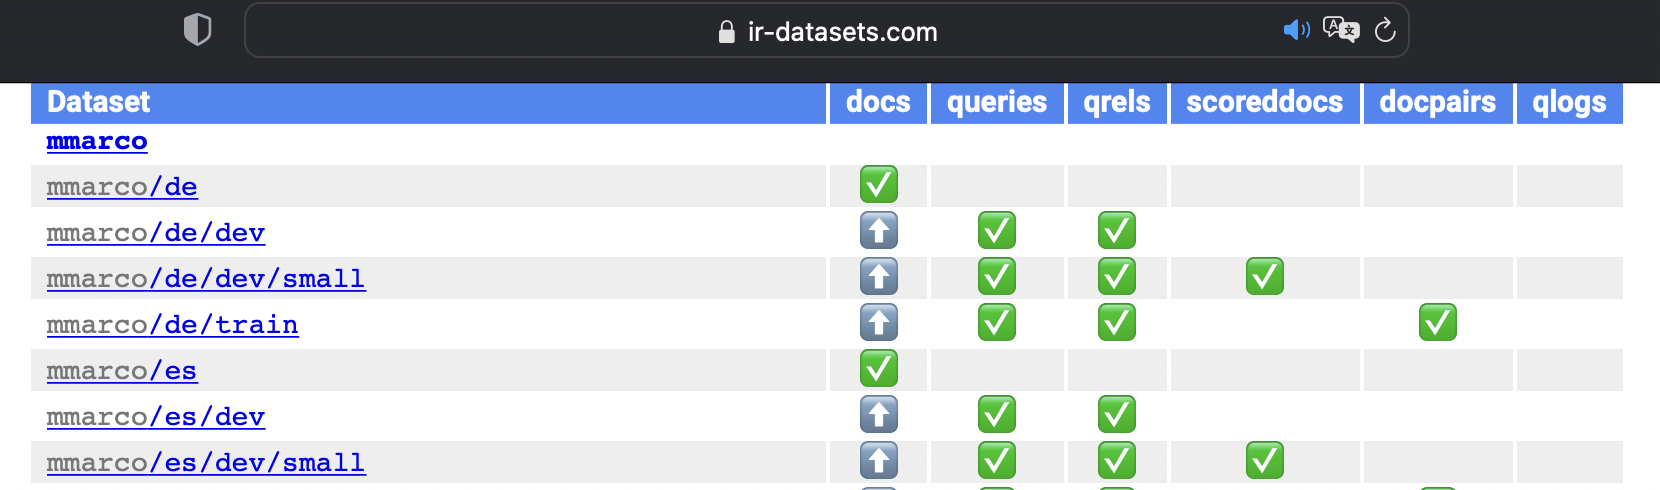
\includegraphics[scale=0.5]{ir-dataset.png}}
		
	\end{frame}
	
		%------------------------------------------------
	% ¿Qué necesito para poder evaluar?
	\begin{frame}
		
		\frametitle{Para poder evaluar ...}
				
		\textcolor{purple}{¿Cómo se pudiese evaluar un sistema?}\\[2mm]
		
		\only<2>{
		R/: Estableciendo relaciones entre la información recuperada y la no recuperada, ambos conjuntos importantes para satisfacer la consulta.}
		
	\end{frame}
	
	%------------------------------------------------
	% Matriz de confusión
	\begin{frame}
		
		\frametitle{Matriz de confusión}
		
		\begin{alertblock}{}
			Herramienta intuitiva para medir el rendimiento de un clasificador.
		\end{alertblock}
		
		\vspace{1\baselineskip}
		Un MRI puede considerarse un clasificador puesto que dada una consulta determina si cada elemento del conjunto de datos la satisface o no.
		
		\pause
		\vspace{2\baselineskip}
		\centering
		\only<2>{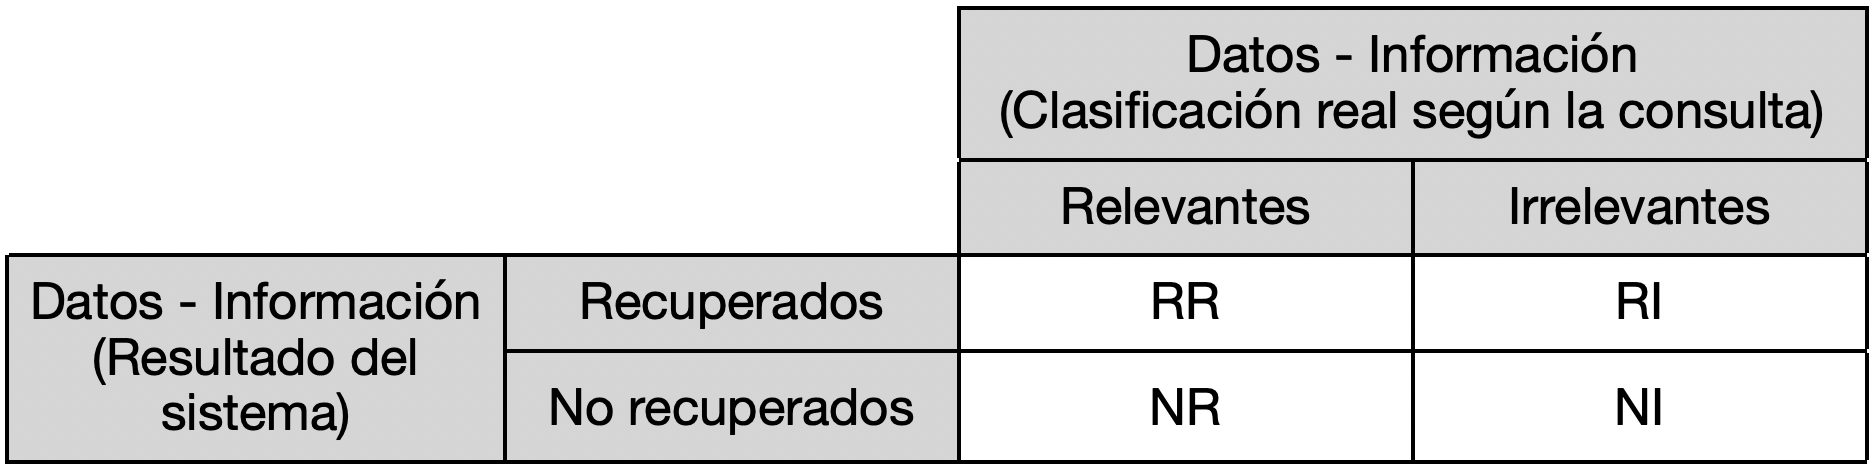
\includegraphics[scale=0.4]{matriz-confusion.png}}
		
	\end{frame}
	
	%------------------------------------------------
	% Interpretación de la matriz de confusión
	\begin{frame}
		
		\frametitle{Interpretación de la matriz de confusión}
		
		\centering
		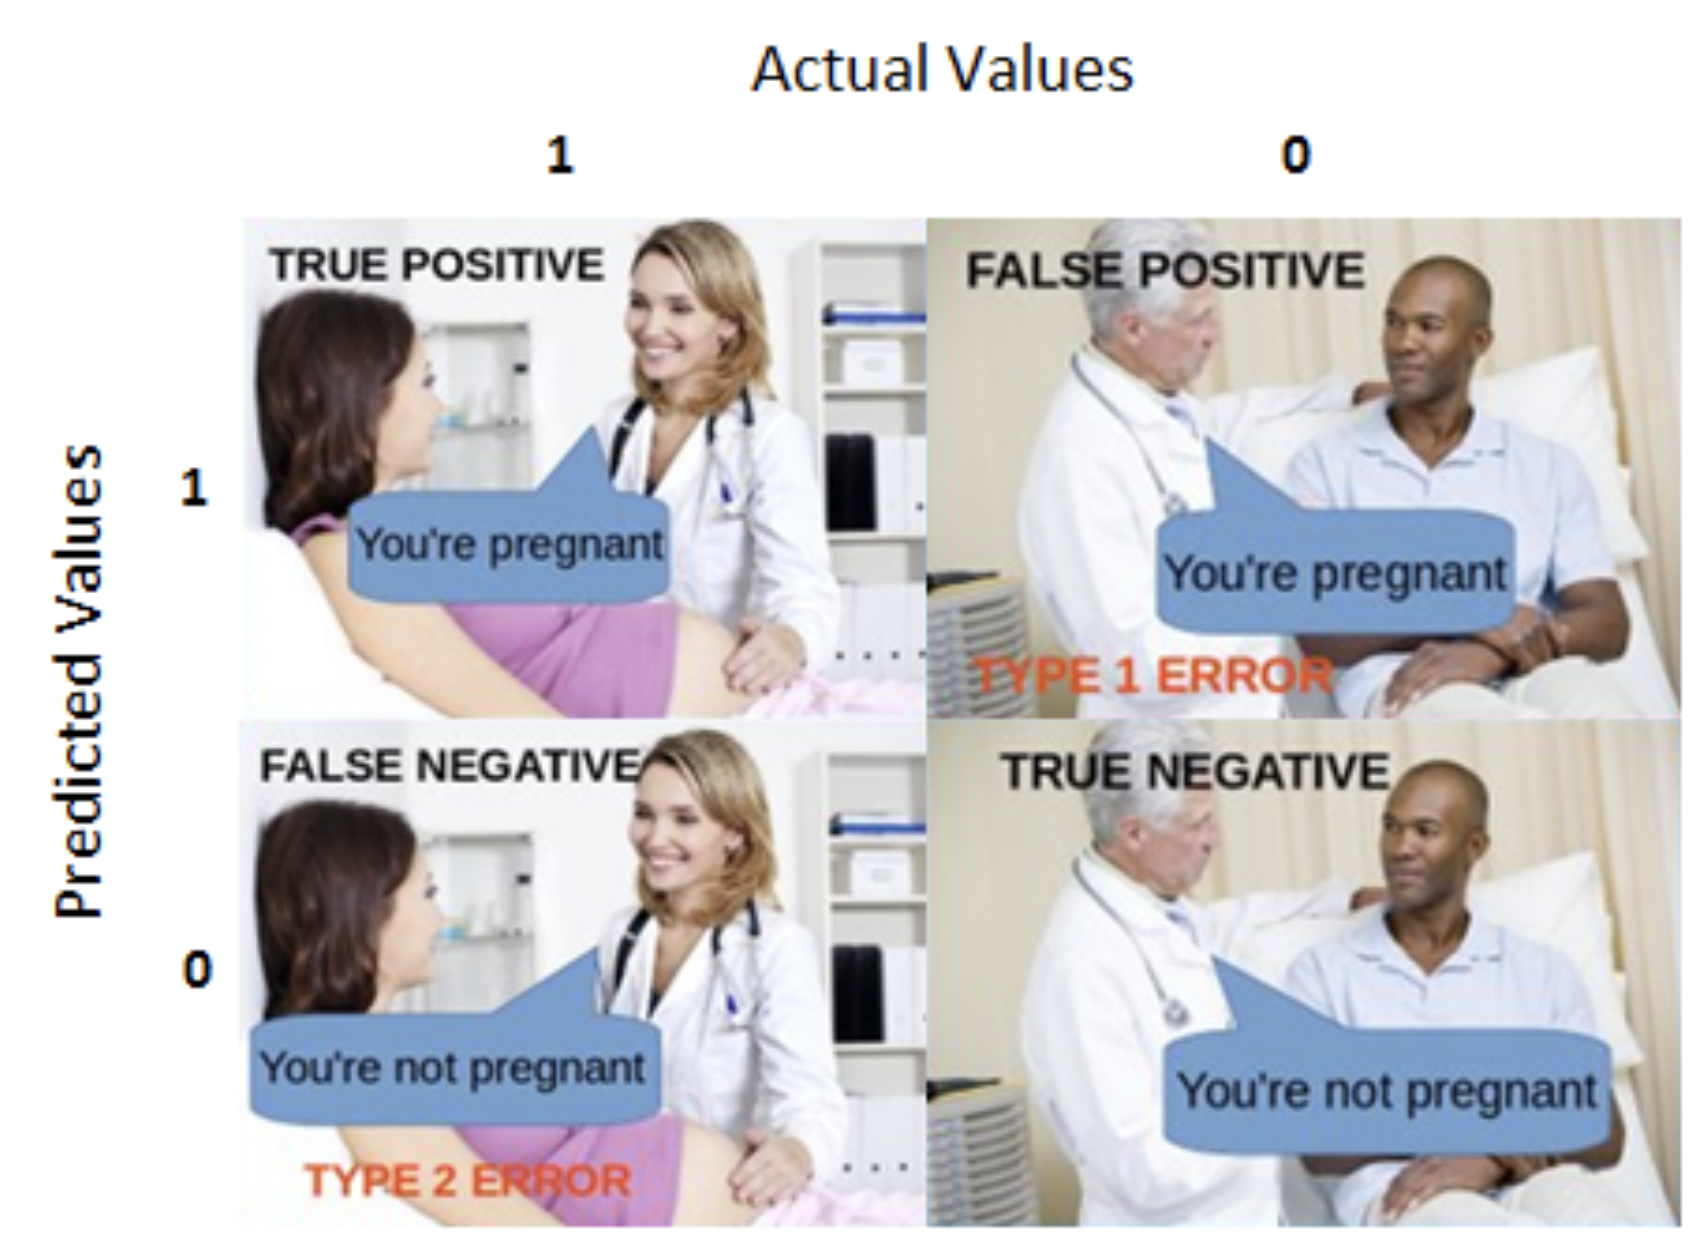
\includegraphics[scale=0.35]{m2.png}
		
	\end{frame}
	
	%------------------------------------------------
	% SRI + Matriz de confusión
	\begin{frame}
		
		\frametitle{SRI + Matriz de confusión}
		
		\begin{minipage}{.4\textwidth}
			\only<1>{
				\hspace{1cm}
			}
			\only<2->{
				\begin{venndiagram2sets}[
					labelA={}, labelB={},
					labelOnlyA={\textbf{REL}}, labelOnlyB={\textbf{REC}}, 
					labelAB={\textbf{RR}},
					labelNotAB={\textbf{NN}}
					]
					\setpostvennhook{
						\draw[<-] (labelOnlyA) -- ++(100:2.5cm) node[above,text width=4cm,align=flush left] {Conjunto de informaciones relevantes};
						\draw[<-] (labelOnlyB) -- ++(90:2cm) node[above,text width=4cm,align=flush right] {Conjunto de informaciones recuperadas};
						\draw[<-] (labelAB) -- ++(-50:3cm) node[below,text width=4cm,align=flush left] {Conjunto de informaciones relevantes recuperadas};
						\draw[<-] (labelNotAB) -- ++(-90:1cm)
						node[below,text width=4cm,align=flush left]
						{Conjunto de informaciones no relevantes no recuperadas};
					}
				\end{venndiagram2sets}
			}
		\end{minipage}%
		\begin{minipage}{.7\textwidth}
			
			\only<1->{
				\begin{figure}[l]
					\centering
					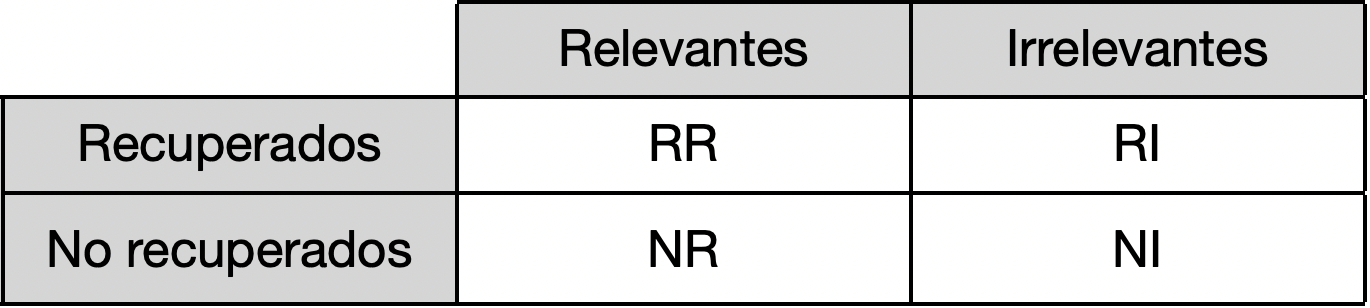
\includegraphics[scale=0.35]{matriz-peq.png}
				\end{figure}
			}
			
			\only<3>{
				\vspace{2\baselineskip}
				
				$$ RR = REL \cap REC $$
				$$ RI = REC \setminus RR $$
				$$ NR = REL \setminus RR $$
				$$ NI = NN $$
			}
			
		\end{minipage}%

	\end{frame}
	
	%------------------------------------------------
	% Medidas de evaluación
	\begin{frame}
		
		\frametitle{Medidas de evaluación}
		
		Tipos de medidas de evaluación:
		
		\begin{itemize}
			\item Objetiva
				\only<2>{
					\begin{itemize}
						\item Precisión
						\item Recobrado
						\item F
						\item F1  
						\item R-Precisión
						\item Proporción de fallo
					\end{itemize}
				}
				
			\item Subjetiva
			
		\end{itemize}
		
	\end{frame}
	
	%------------------------------------------------
	% Medida objetiva: Precisión
	\begin{frame}
		
		\frametitle{Medida objetiva: Precisión}
		
		\begin{figure}[tl]
			\centering
			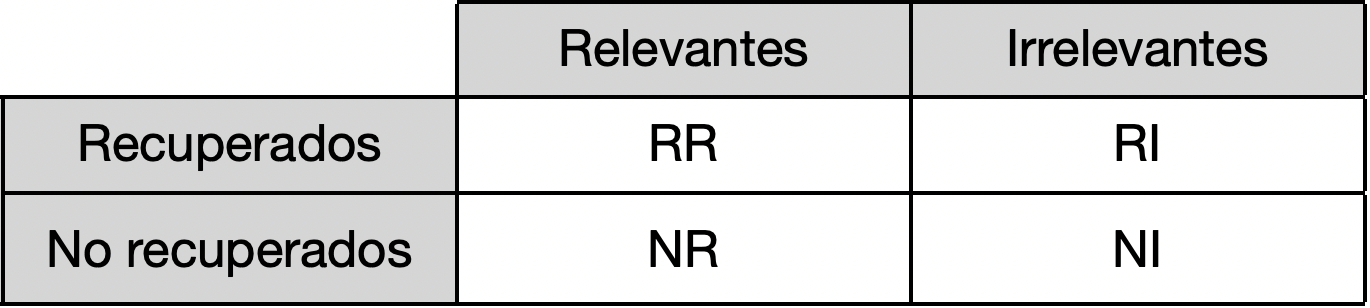
\includegraphics[scale=0.35]{matriz-peq.png}
		\end{figure}
		
		\vspace{2\baselineskip}
		
		\centering
		Fracción de información recuperada que es relevante
		$$P = \frac{|RR|}{|RR \cup RI|}$$
		
		La precisión usualmente tiende a decrecer cuando la información recuperada aumenta
		
		\pause
		\vspace{3\baselineskip}
		\textcolor{purple}{¿Cómo asegurar en un SRI que se cumpla $P=1$?}
		% R/: Devolver solo un dato del cual me asegure que es relevante.
		
	\end{frame}
	
	%------------------------------------------------
	% Medida objetiva: Recobrado
	\begin{frame}
		
		\frametitle{Medida objetiva: Recobrado}
		
		\begin{figure}[tl]
			\centering
			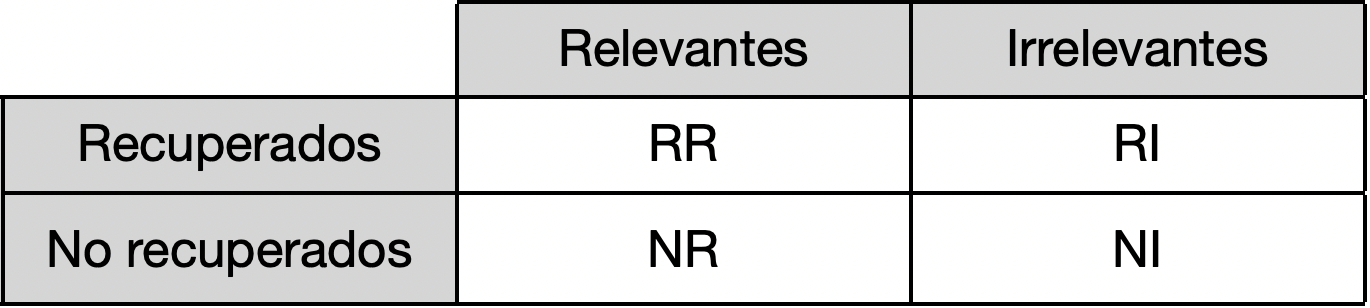
\includegraphics[scale=0.35]{matriz-peq.png}
		\end{figure}
		
		\vspace{2\baselineskip}
		
		\centering
		Fracción de información relevante que fue recuperada
		$$R = \frac{|RR|}{|RR \cup NR|}$$
		
		Esta medida es una función no decreciente para la cantidad de información recuperada
		
		\pause
		\vspace{3\baselineskip}
		\textcolor{purple}{¿Cómo asegurar en un SRI que se cumpla $R=1$?}
		% R/: Devolver todos los datos.
		
	\end{frame}
	
	%------------------------------------------------
	% Precisión VS Recobrado
	\begin{frame}
		
		\frametitle{Precisión VS Recobrado}
		
		\centering
		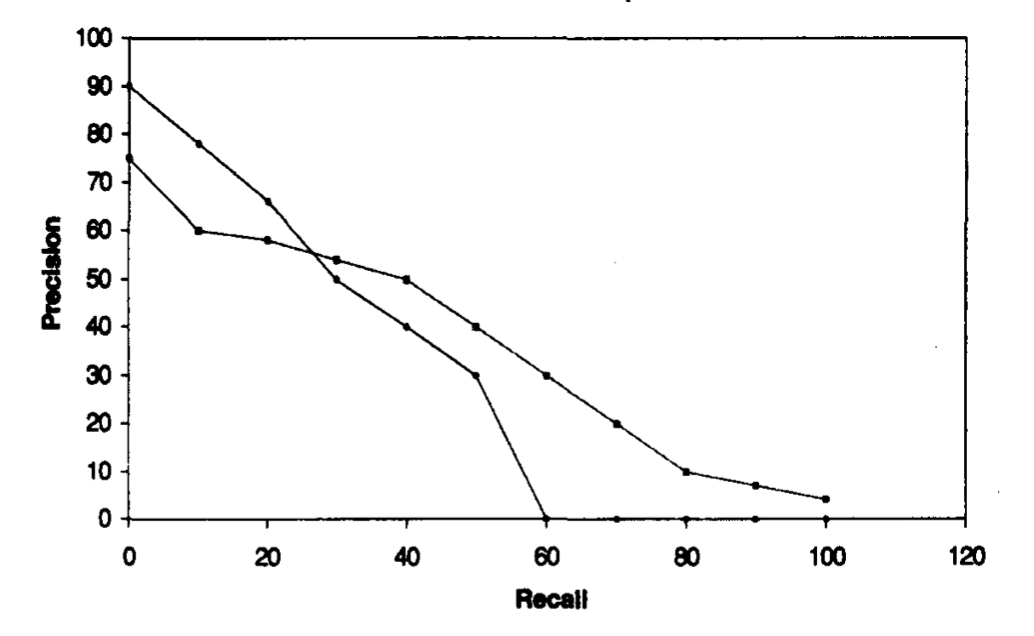
\includegraphics[scale=0.45]{comparacion.png}
		
		\only<1>{
			\begin{itemize}
				\item Si $P=1$ entonces toda la información recuperada es relevante
				\item Si $R=1$ entonces toda la información relevante fue recuperada
				\item Las medidas se compensan (no son inversamente proporcionales)
			\end{itemize}
		}
		
		\only<2-3>{
			\begin{itemize}
				
				\item El \textbf{Recobrado} tiene valor $1$ si se recupera toda la información sin importar la consulta, resultando así una baja \textbf{Precisión}
				\item Idílicamente se desea $P=R=1$ pero pocas veces se logra. Entonces, \textcolor{purple}{¿qué hacer para intentar acercarse a la igualdad?}
				\only<3>{
					\item[] R/: Se intenta obtener un alto valor del \textbf{Recobrado} tolerando una pequeña cantidad de falsos positivos (RI)
				}
			\end{itemize}
		}

	\end{frame}
	
	%------------------------------------------------
	% Medida objetiva: Medida F
	\begin{frame}
		
		\frametitle{Medida objetiva: F}
		
		Establece una métrica a partir de la Precisión (P) y el Recobrado (R), permitiendo enfatizar una medida sobre otra
		
		$$
			F = 
			\frac{(1 + \beta^2)PR}{\beta^2 P + R} 
			% = \frac{1 + \beta^2}{\frac{1}{P} + \frac{\beta^2}{R}} 
		$$ 
		
		\vspace{2\baselineskip}
		\begin{itemize}
			\item $\beta = 1$: Igual peso o énfasis para la Precisión y el Recobrado
			\item $\beta > 1$: Mayor peso o importancia a la Precisión
			\item $\beta < 1$: Mayor peso o importancia al Recobrado
		\end{itemize}
		
	\end{frame}
	
	%------------------------------------------------
	% Medida objetiva: Medida F1
	\begin{frame}
		
		\frametitle{Medida objetiva: F1}
		
		Caso especial de la medida F cuando $\beta = 1$. Es una medida que equipara la Precisión y el Recobrado.
		
		$$
			F1 
			= \frac{2PR}{P+R}
			% = \frac{2}{ \frac{1}{P} + \frac{1}{R} }
		$$
		
		\vspace{2\baselineskip}
		Esta medida toma valor alto cuando la Precisión y el Recobrado son altos, lo que puede interpretarse como un esfuerzo por encontrar el mejor compromiso entre Precisión y Recobrado. 
		
	\end{frame}
	
	%------------------------------------------------
	% Dificultades con la Presición y el Recobrado
	\begin{frame}
		
		\frametitle{Dificultades con la Precisión y el Recobrado}
		
		\begin{itemize}
			\item El conjunto de documentos irrelevantes no es tenido en cuenta.
			
			\pause 
			
			\item La Precisión se indefine cuando no se recupera ninguna información.
			
			\item El  Recobrado se indefine cuando no hay información relevante.
			
			\pause 
			
			\item Se necesita del juicio de expertos tanto para aplicar las medidas e interpretarlas como para crear las colecciones de pruebas.
			
			\item Evaluar el sistema requiere un gran conjunto de consultas y, aun así, no se garantiza el rendimiento del sistema si las métricas arrojaron buenos resultados.
			
			\item La Precisión y el Recobrado, así como F y F1, no toman en cuenta el orden de los resultados que satisfacen la consulta.
		\end{itemize}
		
	\end{frame}
	
	%------------------------------------------------
	% Medida objetiva: Medida R-Precisión
	\begin{frame}
		
		\frametitle{Medida objetiva: R-Precisión}
		
		\begin{minipage}{.5\textwidth}
			
			Calcula la Precisión hasta la posición $k$ del \emph{ranking}
			$$P = \frac{|RR|}{|RR \cup RI|}$$
			\hspace*{2cm}R-Precisión$_7 = \frac{4}{7} \approx 0.57$
			
		\end{minipage}%
		\begin{minipage}{.6\textwidth}
			
			\begin{table}[ht]
			
			\begin{tabular}{|c|c|c|}
				\hline \multirow{2}{1cm}{Orden} 
				& \multicolumn{1}{p{2cm}|} {\centering ID Dato \\ recuperado} 
				& \multicolumn{1}{p{1.5cm}|} {\centering ¿Es \\ relevante?}
				\tabularnewline \hline
				1                        & 456                        & X                        \\ \hline
				2                        & 276                        & X                        \\ \hline
				3                        & 578                        &                          \\ \hline
				4                        & 309                        & X                        \\ \hline
				5                        & 160                        &                          \\ \hline
				6 						& 437 						 & X 						\\ \hline
				7                        & 890                        &                          \\ \hline \hline \hline
				8                        & 426                        &                          \\ \hline
				9                        & 213                        &                          \\ \hline
				10                       & 457                        & X                        \\ \hline
				11                       & 409                        & X                        \\ \hline
				12                       & 806                        &                          \\ \hline
				13                       & 408                        &                          \\ \hline
				14                       & 836                        &                          \\ \hline
			\end{tabular}
			\end{table}
			
		\end{minipage}%
		
	\end{frame}
	
	%------------------------------------------------
	% Medida objetiva: Medida Proporción de fallo
	\begin{frame}
		
		\frametitle{Medida objetiva: Proporción de fallo}
		
		\begin{minipage}{.5\textwidth}
			
			Toma en cuenta la cantidad de información irrelevante en el \emph{ranking} con respecto al total de irrelevantes
			$$Fallout_k = \frac{\text{cantidad de datos irrelevates en los primero k}}{\text{total de datos irrelevantes}}$$
			
			\vspace{3\baselineskip}
			
			Por ejemplo, si el total de información irrelevante es 100 y se desea computar la métrica para el $ranking = 7$, entonces
			
			$$Fallout_7 = \frac{3}{100} = 0.03$$
			
		\end{minipage}%
		\begin{minipage}{.6\textwidth}
			
			\begin{table}[ht]
				
				\begin{tabular}{|c|c|c|}
					\hline \multirow{2}{1cm}{Orden} 
					& \multicolumn{1}{p{2cm}|} {\centering ID Información \\ recuperada} 
					& \multicolumn{1}{p{1.5cm}|} {\centering ¿Es \\ relevante?}
					\tabularnewline \hline
					1                        & 456                        & X                        \\ \hline
					2                        & 276                        & X                        \\ \hline
					3                        & 578                        &                          \\ \hline
					4                        & 309                        & X                        \\ \hline
					5                        & 160                        &                          \\ \hline
					6 						& 437 						 & X 						\\ \hline
					7                        & 890                        &                          \\ \hline \hline \hline
					8                        & 426                        &                          \\ \hline
					9                        & 213                        &                          \\ \hline
					10                       & 457                        & X                        \\ \hline
					11                       & 409                        & X                        \\ \hline
					12                       & 806                        &                          \\ \hline
					13                       & 408                        &                          \\ \hline
					14                       & 836                        &                          \\ \hline
				\end{tabular}
			\end{table}
			
		\end{minipage}%
		
	\end{frame}
	
		%------------------------------------------------
	% Medidas de evaluación
	\begin{frame}
		
		\frametitle{Medidas de evaluación}
		
		Tipos de medidas de evaluación:
		
		\begin{itemize}
			\item Objetiva
			\only<1>{
				\begin{itemize}
				\item Precisión
				\item Recobrado
				\item F
				\item F1  
				\item R-Precisión
				\item Proporción de fallo
				\end{itemize}
			}
		
			\item Subjetiva
			\only<2>{
				\begin{itemize}
					\item Proporción de novedad
					\item Proporción de cobertura
					\item Esfuerzo del usuario
					\item Tiempo de respuesta
					\item Forma de presentación
				\end{itemize}
			}
			
		\end{itemize}
		
	\end{frame}
	
	%------------------------------------------------
	% Medidas subjetivas de evaluación
	\begin{frame}
		
		\frametitle{Medidas subjetivas de evaluación}
		
		\begin{itemize}
			\item Proporción de novedad \\
			\only<2->{Proporción entre la información recuperada desconocida por el usuario y la información relevante recuperada. \\[2mm]}
			
			\item Proporción de cobertura \\
			\only<3->{Proporción entre la cantidad de información recuperada relevante conocida por el usuario y la cantidad de información relevante desconocida por el usuario. \\[2mm]}
			
			\item Esfuerzo del usuario \\
			\only<4->{Trabajo requerido por el usuario en la formulación de consultas, guiado por la búsqueda y la visualización del resultado. \\[2mm]}
			
			\item Tiempo de respuesta \\
			\only<5->{Intervalo de tiempo entre la especificación de la consulta y la presentación de los resultados. \\[2mm]}
			
			\item Forma de presentación \\
			\only<6->{Formato de presentación de los resultados.}
				
		\end{itemize}
		
	\end{frame}
	
	%------------------------------------------------
	% Break
	\begin{frame}
		\centering
		
\includegraphics[height=\paperheight]{break-1.png}
	\end{frame}


	%------------------------------------------------
	% 
	\begin{frame}
		
		\frametitle{Mejorando los resultados encontrados}
		
		
		Para los usuarios es difícil plantear las consultas de modo que expresen sus necesidades informativas. 
		
		\vspace{1\baselineskip}
		Muchas veces los SRI no logran dar respuesta a la necesidad de información del usuario.
		
		\pause
		\vspace{3\baselineskip}
		\textcolor{purple}{¿Cómo puede el usuario ``ayudar'' al sistema a mejorar las búsquedas?} \\
		\textcolor{purple}{¿Cómo puede el sistema ``mejorar'' las búsquedas?}		
		
	\end{frame}
	
	%------------------------------------------------
	% Retroalimentación
	\begin{frame}
		
		\frametitle{Retroalimentación}
		
		\begin{alertblock}{}
			Mecanismo en que cierta proporción de la salida de un sistema se redirige a la entrada para controlar su comportamiento.
		\end{alertblock} 

		\vspace{2\baselineskip}
		Algoritmo clásico: 
		
		\begin{enumerate}
			\item El usuario plantea la consulta
			\item El SRI devuelve un conjunto de información
			\item El usuario selecciona la información que considera relevante 
			\item El sistema obtiene una mejor representación de las necesidades del usuario utilizando esa información
		\end{enumerate}
		
		\pause
		\vspace{2\baselineskip}
		\textcolor{purple}{¿Cómo puede el usuario ``indicar'' la información relevante recuperada por el sistema?}		
		
	\end{frame}
	
	%------------------------------------------------
	% Modelos vistos en clase
	\begin{frame}
		
		\frametitle{Modelos vistos en clase}
		
		\begin{itemize}
			\item Modelo Booleano \\[2mm]
			\item Modelo Vectorial \\[2mm]
			\item Modelo Probabilístico 
		\end{itemize}
		
	\end{frame}
	
	%------------------------------------------------
	% Retroalimentación en el MRI Vectorial
	\begin{frame}
		
		\frametitle{Retroalimentación en el MRI Vectorial}
		
		\textbf{Idea: } Encontrar un vector consulta $\vec{q}$ que maximice la similitud con la información relevante y minimice la similitud con la información no relevante. \\[3mm]
		
		\only<1>{
			\textbf{Consideración: } Los vectores relevantes a una consulta son similares y tienen una diferencia notable con respecto a los no relevantes. \\[3mm]
		}
		
		\only<2->{
			Si se tiene que: \\
			$C_r$ : conjunto de información relevante \\
			$C_{nr}$ : conjunto de información no relevante \\
			Entonces:
			$$\vec{q}_{opt} = arg max( sim(\vec{q}, C_r) - sim(\vec{q}, C_{nr}) )$$
		}
		
		\only<3>{
			Utilizando la distancia coseno entre los vectores de la consulta y los datos, queda:
				$$
					\vec{q}_{opt} = 
						\frac{1}{|C_r|} \sum_{\vec{d}_j \in C_r} \vec{d}_j 
						- \frac{1}{|C_{nr}|} \sum_{\vec{d}_j \in C_{nr}} \vec{d}_j 
				$$
		}
		
	\end{frame}
	
	%------------------------------------------------
	% Visualización
	\begin{frame}
		
		\frametitle{Visualización de $\vec{q}_{opt}$}
		
		Intuitivamente, $\vec{q}_{opt}$ es el vector diferencia entre los centroides de los datos relevantes y los no relevantes.\\[3mm]
		
		\centering
		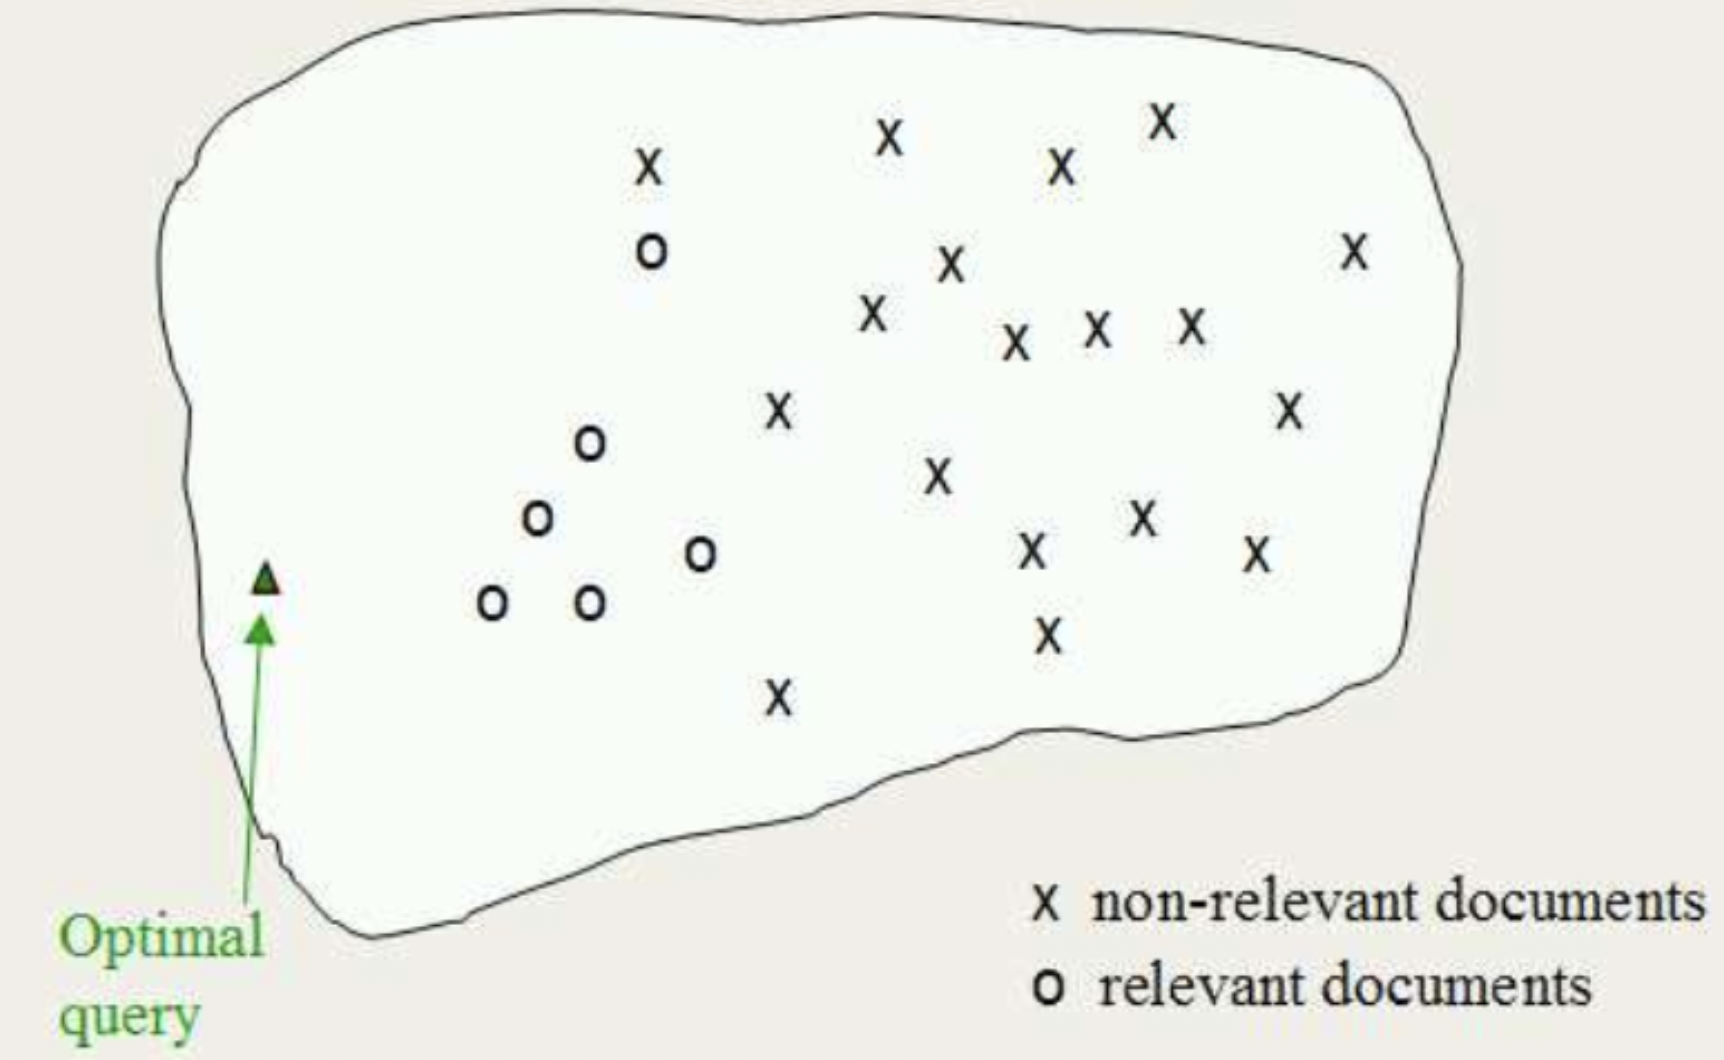
\includegraphics[scale=0.3]{q1.png}
		
	\end{frame}
	
	%------------------------------------------------
	% Algoritmo de Roccio
	\begin{frame}
		
		\frametitle{Algoritmo de Rocchio}
		
		Se parte de que dada una consulta solo se conoce parcialmente el conjunto de los datos relevantes (factor $\beta$) y los no relevantes (factor $\gamma$). \\[2mm]
		
		Se tenía que 
		$$
		\vec{q}_{opt} = 
		\frac{1}{|D_r|} \sum_{\vec{d}_j \in D_r} \vec{d}_j 
		- \frac{1}{|D_{nr}|} \sum_{\vec{d}_j \in D_{nr}} \vec{d}_j 
		$$
		
		Luego,
		$$
			\vec{q}_{modificado} = 
				\alpha \vec{q} 
				+ \frac{\beta}{|C_r|} \sum_{\vec{d}_j \in C_r} \vec{d}_j 
				- \frac{\gamma}{|C_{nr}|} \sum_{\vec{d}_j \in C_{nr}} \vec{d}_j 
		$$
		
		\vspace{1\baselineskip}
		
		\only<2>{
			Consideraciones:
			\begin{itemize}
				\item $\beta$ y $\gamma$ pueden tener valores altos para cuando los conjuntos de datos sean grandes.
				
				\item Se puede asumir que $\beta > \gamma$ debido a la importancia de los datos relevantes sobre los no relevantes.
				
				\item Generalemente $\alpha = 1$, $\beta = 0.75$ y $\gamma = 0.15$.
			\end{itemize}
		}
		
	\end{frame}
	
	%------------------------------------------------
	% Visualización del Algoritmo de Rocchio 
	\begin{frame}
		
		\frametitle{Visualización del Algoritmo de Rocchio}
		
		\centering
		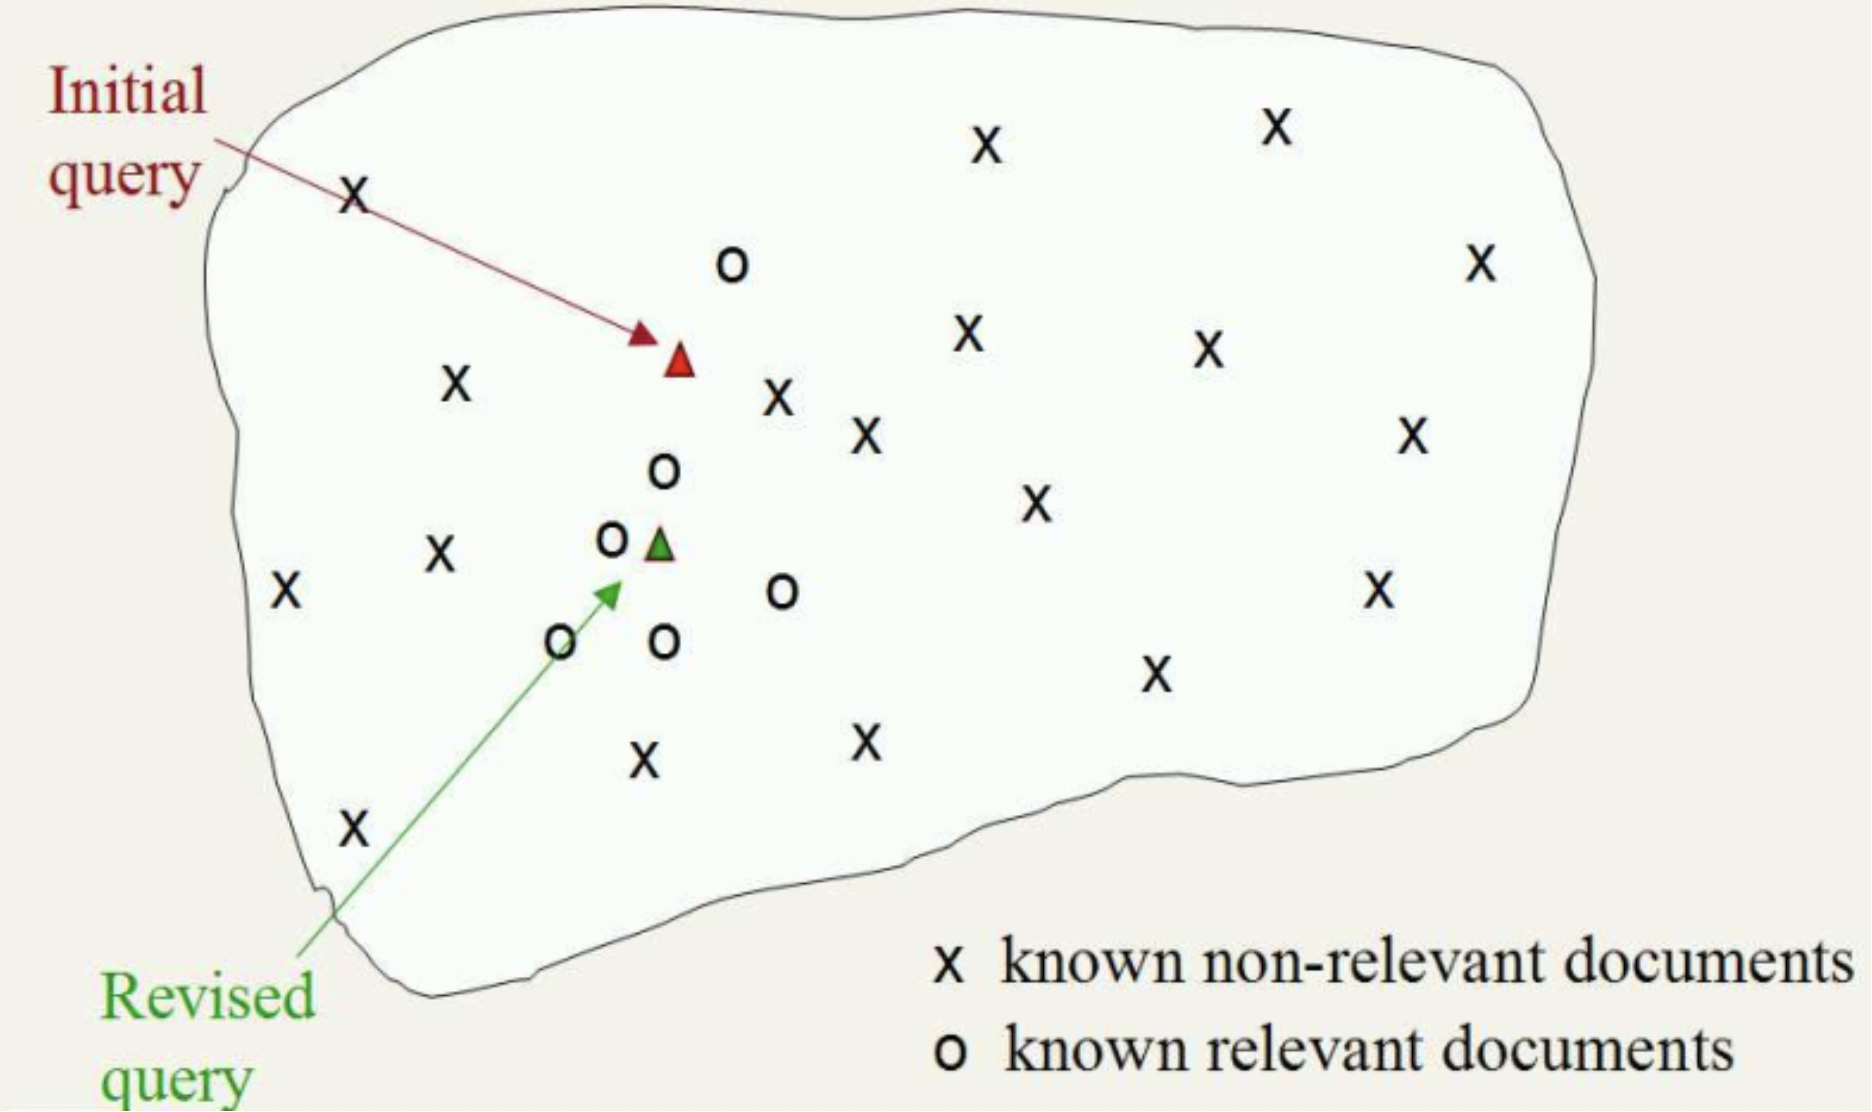
\includegraphics[scale=0.35]{q2.png}
		
	\end{frame}
	
	%------------------------------------------------
	% Retroalimentación en el MRI Vectorial
	\begin{frame}
		
		\frametitle{Retroalimentación en el MRI Probabilista}
		
		Se conoce que:
		$$sim(d_j, q) = \sum_{i = 1}^{n} w_{i, q} \times w_{i, j} \times (\log \frac{p(t_i|R)}{1 - p(t_i|R)} + \log \frac{1 - p(t_i|\overline{R})}{p(t_i|\overline{R})})$$
		
		donde:
		\begin{itemize}
			\item $p(t_i|R) = 0.5$
			\item $p(t_i|\overline{R}) = \frac{n_i}{N}$ \\[3mm]
		\end{itemize}
		
		\pause
		\vspace{2\baselineskip}
		\textbf{Idea: } Construir un clasificador binario. Puede ser el modelo probabilístico de Naive-Bayes \\[3mm]
		% Recordar que Naive-Bayes sume independencia entre las variables, por lo que la probabilidad condicional se convierte en una multiplicación.
		
	\end{frame}
	
	%------------------------------------------------
	% Retroalimentación en el MRI Vectorial
	\begin{frame}
		
		\frametitle{Retroalimentación en el MRI Probabilista}
		
		Luego, los términos puede calcularse como:
		\begin{align*}
			p(t_i|R) &= \frac{|VR_{t_i}|}{|VR|} \\
			p(t_i|\overline{R}) &= \frac{df_{t_i} - |VR_{t_i}|}{N - |VR|}
		\end{align*}
		
		
		\begin{itemize}
			\item $N$ : tamaño del conjunto de datos
			\item $df_{t_i}$ : cantidad de datos que contienen al término $t_i$
			\item $VR$ : conjunto de datos relevantes conocidos
			\item $VR_{t_i}$ : subconjunto de $VR$ que contienen al término $t_i$ \\[3mm]
		\end{itemize}
		
		\pause
		\vspace{2\baselineskip}
		\textcolor{purple}{¿Qué problema tiene el cálculos de los términos $p(t_i|R)$ y $p(t_i|\overline{R})$?}	
		% R/: Necesita un conjunto inicial de documentos relevantes.
		
		
	\end{frame}
	
	%------------------------------------------------
	% Otras formas de aplicar retroalimentación
	\begin{frame}
		
		\frametitle{Otras formas de buscar la retroalimentación}
		
		\begin{itemize}
			\item Pseudo-Retroalimentación \\ 
			Se seleccionan como información relevante los $k$ primeros datos del \emph{ranking} dado como resultado por el sistema y luego se aplica la retroalimentación.
			
			\item Retroalimentación Indirecta \\ 
			Se considera como resultados relevantes aquellos en los que el usuario muestra interés, a partir de los cuales se realiza la retroalimentación. Dicho interés se estima a partir de la captura de información implícita (cantidad de clics, tiempo de lectura, otros).
		\end{itemize}
		
	\end{frame}
	
	%------------------------------------------------
	% Ventajas y desventajas de la retroalimentación
	\begin{frame}
		
		\frametitle{Ventajas y desventajas de la retroalimentación}
		
		\begin{itemize}
			\item Ventajas
			\begin{itemize}
				\item Automatiza el proceso para mejorar la selección de la información relevante.
				
				\item Aumenta la precisión y el recobrado.
			\end{itemize}
			
			\vspace{2\baselineskip}
			
			\item Desventajas
			\begin{itemize}
				\item Pocos usuarios pasan a la segunda vista de los datos paginados, por lo que no es común su interés en participar en la retroalimentación.
				
				\item Es complicado entender por los usuarios la importancia de la retroalimentación.
				
				\item Las consultas generadas por los algoritmos de retroalimentación son muy grandes e ineficientes para los algoritmos de recuperación.
				
			\end{itemize}
		
		\end{itemize}
		
	\end{frame}
	
	%------------------------------------------------
	{
		\setbeamertemplate{background canvas}
		{%
			
\includegraphics[width=\paperwidth,height=\paperheight]{feedback.jpg}
		}
		
		\begin{frame}
		\end{frame}
	}
	
	%------------------------------------------------
	% Mejorando la consulta
	\begin{frame}
		
		\frametitle{Mejorando la consulta}
		
		\textbf{Consulta del usuario:} Necesito información sobre cómo cultivar plantas de rosa mosqueta 
		
		\vspace{4\baselineskip}
				
		\textcolor{purple}{¿Cómo el usuario puede recuperar datos referentes a ``rosa mosqueta'' y ``escaramujo'', si se conoce que ambos términos referencian a la misma flor?}		
		
	\end{frame}
	
	%------------------------------------------------
	% Ejemplo de expansión de consulta
	\begin{frame}
		
		\frametitle{Ejemplo de expansión de consulta}
		
		\centering
		
\includegraphics[scale=0.5]{expansion.png}
		
	\end{frame}
	
	%------------------------------------------------
	% Expansión de consulta
	\begin{frame}
		
		\frametitle{Expansión de consulta}
		
		\begin{alertblock}{}
			Proceso de reformular una consulta para mejorar el rendimiento de las operaciones de recuperación del sistema. Involucra evaluar una consulta y modificarla para que se ajuste a datos adicionales obtenidos de forma automática.
		\end{alertblock}
		
		\vspace{2\baselineskip}
		
		Alternativas: 
		\begin{itemize}
			\item Aumentar el conjunto de términos de la consulta
			\item Variar los pesos de los términos de la consulta			
		\end{itemize}		
		
	\end{frame}
	
	%------------------------------------------------
	% Enfoques de la expansión de la consulta
	\begin{frame}
		
		\frametitle{Enfoques de la expansión de la consulta}
		
		\begin{itemize}
			
			\item Análisis global 
			\begin{itemize}
				\item Uso de fuentes externas como ontologías,  taxonomías, tesauros u otras bases de conocimientos.	
				\item Cada término de la consulta puede aportar sinónimos u otros términos relacionados.
			\end{itemize}
			
			\vspace{2\baselineskip}
			
			\item Análisis local 
			\begin{itemize}
				\item Utiliza solo la información almacenada en la base de datos del sistema.
				\item Los términos a agregar en la consulta son aquellos más ``relacionados'' encontrados en los datos almacenados del sistema. Una alternativa para esto es la matriz de co-ocurrencia.
			\end{itemize}
			
		\end{itemize}
		
	\end{frame}
	
	%------------------------------------------------
	% Bibliografía
	\begin{frame}
		
		\frametitle{Bibliografía}
		
		\begin{itemize}
			\item Baeza-Yates, R. a.-N. (2002). Modern Information Retrieval, cap. 3, 5.
			\item Manning, C. D. (2009). An Introduction to Information Retrieval. Cambridge UP, cap. 8, 9.
		\end{itemize}
		
	\end{frame}
	
	%------------------------------------------------
	% Fin
	\begin{frame}
		\titlepage
	\end{frame}
	
	
	
\end{document} 